%----------------------------------------------------------------------------------------
%	PACKAGE SECTION
%----------------------------------------------------------------------------------------
\documentclass[6pt]{article} %Document font size is 6pt and is an article
\usepackage{multicol}

\usepackage[english]{babel} % English language/hyphenation
\usepackage{amsmath,amsfonts,amsthm} % Math packages
\usepackage{mathtools}
\usepackage[margin=2cm]{geometry}
\usepackage{xcolor}
\usepackage{listings}
\usepackage{url}
\usepackage{mdframed}
\usepackage{graphicx}
\usepackage{caption}
\usepackage{natbib}

\usepackage{fancyhdr} % Custom headers and footers
\pagestyle{fancyplain} % Makes all pages in the document conform to the custom headers and footers
\fancyhead{} % No page header - if you want one, create it in the same way as the footers below
\fancyfoot[L]{} % Empty left footer
\fancyfoot[C]{} % Empty center footer
\fancyfoot[R]{\thepage} % Page numbering for right footer

\setlength\parindent{0.0pt} %No indentation on the paragraphs

%----------------------------------------------------------------------------------------
%	TITLE SECTION
%----------------------------------------------------------------------------------------

\newcommand{\horrule}[1]{\rule{\linewidth}{#1}} % Create horizontal rule command with 1 argument of height

\title{	
\normalfont \normalsize 
\textsc{Department Of Computer Science, University of Bath} \\ [5pt] % Your university, school and/or department name(s)
\textsc{EngD in Digital Entertainment} \\ [5pt] 
\horrule{0.7pt} \\[0.2cm] % Thin top horizontal rule
\Huge A review on crowd simulation and rendering \\ % The assignment title
\vspace{7 mm}
\Large CM50244 \: Computer Animation and Games I \\
\horrule{0.7pt} \\[0.0cm] % Thick bottom horizontal rule
}
\author{Garoe Dorta-Perez \\ \Large Unit Leader: Prof Phil Willis \\}  % Your name\\ 

\begin{document}
\vspace*{\fill}
\begin{center}
	\begin{minipage}{1.0\textwidth}
		\maketitle % Print the title
		\thispagestyle{empty}
	\end{minipage}
\end{center}


%----------------------------------------------------------------------------------------
%	ABSTRACT SECTION
%----------------------------------------------------------------------------------------

\vfill %Space after the title
\begin{abstract}
\normalsize %Make abstract font a big bigger
In this paper we present a survey on crowd simulation techniques.
The whole crowd simulation pipeline is discussed, including: crowd generation, crowd editing, behaviour simulation with path and collision avoidance, and rendering techniques.
First, modelling and rendering classifications are drawn.
Next, for each relevant area or group, a representative paper is chosen, important contributions are outlined, and recent research breakthroughs are given.
\end{abstract}
\vfill %Space after the abstract

\clearpage %Start a new page

%----------------------------------------------------------------------------------------
%	MAIN SECTION
%----------------------------------------------------------------------------------------


\begin{figure}
		\centering
		%\includegraphics[scale=0.2]{images/crowd1}
		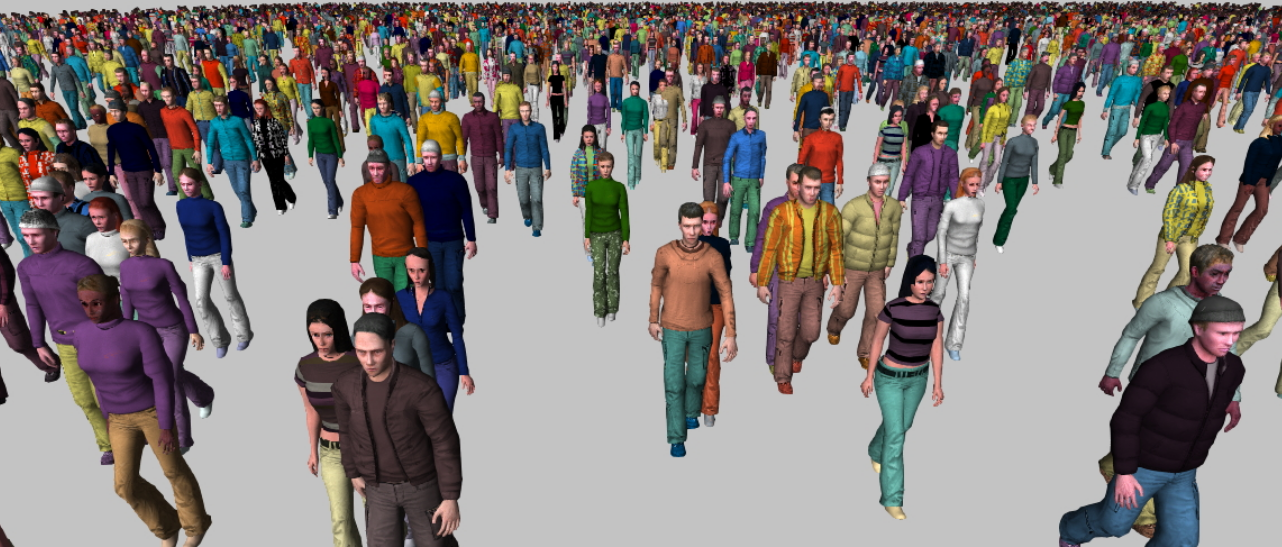
\includegraphics[scale=0.3]{images/crowd2}
		\caption{Animated crowd example, ~\cite{ruiz2013}.}
\end{figure}

\setcounter{page}{1} %Set page number
\columnsep 25.0pt %Column separation
\begin{multicols}{2} %Set for two columns

\section{Introduction}
\label{intro}

%Include why crowd simulation is interesting in films and videogames????
Crowds are encountered frequently, for example, large numbers of people in big shopping areas, during popular sports events or demonstrations.
Non human crowds are quite common as well, such as schools of fish or flocks of birds.
There is a wide range of motives for their simulation.
For instance, in the \textit{film} industry where it is not always possible or economically viable to have a real crowd, in the \textit{video games} industry as a crowd might be required in a virtual world and lastly, in \textit{disaster prevention and management} where they are used to aid the decision making process as simulating the behaviour of a crowd provides new sources of data.\\

A crowd is much more than the collections of individuals that form it.
And as such the behaviour of an individual could affected other crowd members.
History shows how in some cases, crowds of people behave in a well organized manner, while in others its individuals act selfishly, abandoning all social norms.
When simulating this interactions with a na\"ive approach, as the numbers of characters in the crowd increases, the computational cost of the interrelations calculation grows exponentially.\\

This topic has a number of clearly differentiated areas.
Firstly, there is a \textit{crowd generation} problem, a modeller needs user-friendly tools in order to set up a scene in which a crowd is present.
Secondly, the crowd is an evolving entity, so a \textit{crowd dynamics model} is required to govern the behaviour of the crowd over time.
Thirdly, the model should be presented to the user, so a \textit{rendering} stage is needed.\\

Crowd simulation and rendering has been an active research area as early as 1987, with a simulation of flocks of birds by \cite{Reynolds1987}.
The author proved that a coherent global behaviour could be achieved by implementing a number of local rules in each entity.

\section{Classifications}

A clear line can be drawn between real-time simulation (e.g. games) and non real-time simulation (e.g. films).
The requirements for each simulation are quite different and so are the techniques used in each area.
However, with such a broad area, a more detailed exploration is required.
Consequently, each of the stages defined in Section~\ref{intro} will be treated independently.

\subsection{Modelling Classifications}
\label{subsec:ModelClassification}

In order to simulate crowd behaviour a number of approaches have been proposed.
As they share certain features, criteria such as the simulation time or the the size of the modelled crowd can be used for classification.\\

The type of model used for the agents in the crowd can also be used as a criteria.
Therefore, there are \textbf{entity based} simulations, where all individuals are homogeneous, or \textbf{agent based} simulations, where each individual is intelligent and autonomous.
Generally, agent based and entity based systems are used for small and medium size crowds.\\

For big size crowds, due to their challenging nature, \textbf{flow based} simulations are adopted as the most common approach.
In flow based simulations the discrete individual is disregarded in favour of a fluid based approach.
Evidently, this assumption looses effectiveness as the density of entities in the crowd decreases.
This type of simulation is typically used when the crowd reaches a predetermined density threshold, i.e. on dense crowds\\

Lastly, \textbf{hybrid methods} are based on two or more of the aforementioned techniques.
Their advantage lies in choosing the best model according to the situation or even directly mixing characteristics as needed.
For example, using an agent based simulation with low density crowds, and dynamically switching to a flow based simulation if a high density situation occurs.

\subsection{Rendering Classifications}
\label{subsec:RenderingClassification}

Rendering techniques can be classified considering how they perform model reductions, since they have to be able to efficiently render the huge amounts of data needed for crowd simulation.\\

\begin{itemize}
\item \textbf{Dynamic mesh decimation} involves adopting simpler mesh representations.
\item \textbf{Dynamically generated impostors} entails displaying 2D billboards instead of the full model.
\item \textbf{Point-rendering} techniques build multi-resolution representations using point samples from the mesh.
\item Methods to \textbf{achieve variety} are needed, because using ``cloned'' models is a common technique. Since creating unique meshes for each entity in the crowd would be computationally impractical and quite time consuming, a common procedure in rendering crowds is to share the same render model among several entities.
Because this ``cloned'' models are visually undesirable, methods to infuse divergence are required.
\end{itemize}
  

\section{Generating Crowds}
\label{sec:CrowdGen}

Unfortunately, crowd generation has not been researched as deeply as crowd simulation or crowd rendering.
In this stage the initial parameters at which the crowd operates are defined.
For example, crowd size, goals, collision range, minimum/maximum speed, etc.\\

\cite{Ulicny2004} proposed a brush metaphor to manipulate crowds.
The author's technique provides tools in the form of a brush operator(create individuals, change color, etc) and then those tools can be used in the crowd world space.
The entities edited in the crowd will be those in sight in the screen domain.
Therefore, as brush metaphors are common in other areas, an easy to use technique is provided.
However it has certain limitations, such as lack of direct control over crowd behaviour or difficulty to select individuals in cluttered environments.\\

Some of the shortcomings in the previous work were met by \cite{Jordao2014}, whose method utilizes crowd patches.
Such patch areas define the crowd behaviour and can be edited through a sculpting metaphor, while also addressing the problem of populating vast empty areas efficiently.
What is more, crowd motion can be modified on the fly as the patches are editable in real time.
Nonetheless, individual paths cannot be controlled and only linear patch transformation was explored.

\section{Simulating Crowds}

As stated in Section~\ref{intro}, following a na\"ive approach leads to intractable computing times in simulations that handle more than a small sized crowd.
Below we describe in detail the approaches mentioned in Section~\ref{subsec:ModelClassification}. 

\subsection{Entity Based}

\cite{Helbing2000} presented a model where individuals are represented as particles with velocity, mass and forces.
Each entity goals are encoded as values in such components.
The model was designed to replicate pedestrian behaviour in panic situations.
Shortcomings derive from the restricted aim of the simulation, such as difficult per group control and simplistic behaviour.\\

\cite{batty2003} introduced a similar pedestrian model although aimed at simulating carnivals and parades.
The author's model is based on a cellular automata, where an agent step is encoded as moving from the current cell to a neighbour cell.
This technique is constrained to evaluating safety policies and it only has an offline work mode.

\subsection{Agent Based}

\cite{raupp2001} presented a three fold approach to agent based simulations: scripted behaviours, behavioural rules, with events and reactions, and external controls to guide the behaviour.
Controlling the complexity of the behaviours by group settings provides a flexible framework for crowd editing.
Nevertheless, complex individual behaviour was not achieved.\\

\cite{helbing2002} did a complete study of crowd actions in a broad range scenarios, with special attention at panic versus not panic crowd behaviour.
A common pedestrian model applicable to all the situations was derived.\\

More recent techniques add a counterflow paradigm, where agents take into account long distance collision avoidance in addition to trail formation, \cite{heliovaara2012}.
Earlier methods generate unrealistic jams and collision in counterflow situations, that are successfully solved using this technique.
Nevertheless, this model still fails to account for other behaviours, as it is only concerned with counter-flow situations.

\subsection{Flow Based}

\cite{hughes2003} proposed a flow based method to simulate large crowds behaviour based on intelligent fluid flow.
An intelligent fluid tends to prefer certain paths, i.e. avoiding excessive congestive areas, achieving a more complete model for pedestrian simulation.
However, it would not take into account crowd flow in the individual speeds, which prevents lane formation.\\

The previous model was improved by \cite{treuille2006} with the addition of continuum dynamics.
Fixing the aforementioned problems as well as undesirable oscillations in Hughes's model.
Like other flow based models, this technique fails to take into account individual variability.
Moreover, it is limited to have a single common goal for all the characters.

\subsection{Hybrid Models}

\cite{Narain2009} presented an agent-fluid hybrid model.
Each agent has a preferred velocity and a desired path, however on densely populated regions an incomprehensibility flow factor comes into play.
This factor prevents agents from packing together too closely.\\

More recently \cite{lin2014} proposed also an agent-fluid hybrid solution for long-range collision avoidance.
When the density is below a certain threshold a discrete collision avoidance is used,
while above the threshold a fluid based lookahead algorithm controls the behaviour.
This technique shows advanced complex behaviour, such as a large group splitting in two to make space for a smaller group to go through it.
However, in some cases it leads to unnatural groups separations.

\section{Rendering Crowds}

The main obstacle to overcome with crowd rendering is, how to simplify the scene in order to render it in real or at least feasible time.
Hence, the goal in the following techniques is to reduce the computations in the rendering stage.
A common approach consist of applying a model complexity reduction that is still visually unnoticeable.
Below, we present in more detail the techniques commented in Section~\ref{subsec:RenderingClassification}.

\subsection{Dynamic Mesh Decimation}

Progressive meshes were introduced by~\cite{Hoppe1996} as a compressed alternative to traditional meshes.
However, progressive meshes can also be used as a coarser visual representation of the original mesh.
An increase in rendering performance can be accomplished, provided that the decimation calculation is smaller than the rendering gain.
Yet, the coarseness is limited if rendering quality is to be preserved.\\

Building on Hoppe's work, \cite{Hu2009} proposed a GPU implementation for progressive mesh refinement.
Anyhow, the author's implementation is more a feasibility test, rather than a real improvement in performance.

\subsection{Dynamically Generated Impostors}
\label{subsec:DimGenImpostors}

Impostors are 2D pre-computed billboards used in place of full 3D mesh models, thus reducing the cost of the rendering stage, as shown by~\cite{Aubel2000}.
However, when an impostor is rendered to an area larger than the impostor resolution, pixels from the impostor texture become noticeable.\\

%TODO Add drawback
~\cite{Millan2006} presented a GPU impostor implementation, which also used pseudo-instancing for further performance gains~\cite{zelsnack2004glsl}.
Yet, their implementation is only designed for a single GPU.\\

More recent advances were made by~\cite{Ghiletiuc2013} with a client-server impostor implementation in mobile devices.
Nevertheless, the bulk of the computation was still performed on the server side.

\subsection{Point-Rendering}

Point rendering uses a point cloud subset from the mesh model to reduce the complexity of the meshes in the crowd.
Using less points as the camera moves further away from the model.
\cite{Wand2002} showed that by using multi-resolution point sample rendering in key frame animations, the rendering time becomes independent from the complexity of the geometric model.\\

~\cite{Larkin2010} presented a point-rendering method that achieved real-time rendering by limiting the resources of the whole crowd, and sharing them with a level of detail value determined by a Delaunay triangulation. 
Each vertex in the triangulation has a density value that is used to calculate the number of points to render.
With small and medium crowds this technique works reasonably well.
However, with very large crowds the resources allocated for each instance can be insufficient.

\subsection{Achieving Variety}

There has been research into applying color variety, height change, accessory addition and animation variety to copies of individuals.
As it is an inexpensive method to create the illusion of a varied crowd when the actual crowd is generated using ``clones'' .
Moreover, this techniques rely on instancing, which is a desirable property,~\cite{zelsnack2004glsl}.\\

Crowds in specific situations has been simulated, for example \cite{deHeras2005} worked with a virtual Roman crowd in an urban environment.
In this paper they avoided computing each character’s mesh deformation.
Instead a precomputed deformed mesh was calculated for each frame. 
As well as applying hardware accelerated color modulation on instances of the same mesh model.\\

\cite{ruiz2013} proposed a memory efficient method to generate new characters by varying skin color, clothes and body size.
The author's method involves a preprocessing stage and a run time stage.
In the first stage, assets are generated from the individuals, including texture maps, new animations, etc.
This phase is done per body part mesh to increase asset reusability.
While on the second step new characters are animated using the previously generated assets.
However, the method is still not fully automatic and it needs pregenerated rigs.
% Topics to look for in papers are to be added in this area 
%- Color modulation
%- Texture variation
%- Shape deformation
%- Outfit creation
%- Animation diversity

\section{Conclusion}
We have seen an overview of the research techniques applied in crowd generation, simulation and rendering.
The generation and editing areas are still not sufficiently mature as to provide easy to use tools.
However, important advances have been made, e.g. the crowd brush metaphor or the crowd patches discussed in Section~\ref{sec:CrowdGen}.\\

On the simulation side, there is a clear trend to abandon entity based simulations in favour of agent based simulations and hybrid approaches.
Flow based simulations sacrifices too much detail, nevertheless hybrid simulations tend to address the issue.
However, this methods are still not general enough.
Besides, artificial outcomes are generated under certain input parameters.\\

On the rendering area, LOD techniques have been refined into research areas on their own.
Such as progressive meshes or point cloud rendering.
The use of instances with automatic colour, height or accessories variation optimizes the rendering stage.
Moreover, most of these techniques produce reasonable results without manual intervention.
Nonetheless this techniques still do not implement highly realistic interactive rendering.\\

In all these areas, a lot of processing previously done by the CPU have been moved to the GPU, \cite{Hu2009}, \cite{Millan2006}.
This line of research has produced significant performance gains.
However, a behaviourally complex, real-time simulation with easy editing and high quality rendering is still unachievable with the current techniques.

\bibliographystyle{apalike} %Close to Harvard style
\bibliography{template} %Include template.bib bibliography file
\end{multicols}
\end{document}
